\input{preamble_2}
%-----------------------------------------------------------------------------------------------------------------------
% 文章開始
\title{ BOP2: Bayesian optimal design for phase II clinical trials with simple and complex endpoints\\BOP2：具有簡單和複雜終點的II期臨床試驗的貝葉斯最優設計}
\author{{周昱宏}}
\date{{\TT \today}}
\begin{document}
\maketitle
\fontsize{12}{22 pt}\selectfont
\doublespacing

\section{abstract}

我們提出了一種靈活的貝葉斯最佳第二期臨床試驗設計（BOP2），該設計能夠在一個統一框架下處理簡單（如二元終點）和複雜（如有序、嵌套和共同主要終點）終點。我們使用狄利克雷-多項式模型來適應不同類型的終點。在每個中期分析時，通過評估感興趣事件的後驗機率集合來做出繼續或停止試驗的決策，該決策優化目標是最大化檢定力或在虛無假設下最小化患者數量。與其他現有的貝葉斯設計不同，BOP2設計能夠明確控制I型誤差率，從而縮小了貝葉斯設計與頻率學派設計之間的差距。此外，BOP2設計的停止邊界可以在試驗開始前就確定，這些特點使得BOP2設計易於被各類用戶和監管機構接受和實施。模擬研究顯示，BOP2設計在運行特性上表現出較高的檢測力和較低的誤終止試驗風險，優於一些現有的貝葉斯第二期設計。

重點:

這段文字描述了BOP2設計的幾個關鍵點：

靈活性：BOP2設計能夠在一個統一的框架下處理多種類型的臨床試驗終點，無論這些終點是簡單的二元變量還是複雜的有序、嵌套或共同主要終點。

數學模型：BOP2設計使用了狄利克雷-多項式模型來處理不同終點類型的數據。這種模型能夠適應各種複雜情況，如多個變量之間的關聯。

決策過程：在試驗過程中，研究者通過期中分析來決定是否繼續試驗。這個決策是基於後驗機率的評估，目的是在最大化檢測效果的同時，避免讓過多患者參與一個可能無效的試驗。

I型誤差控制：BOP2設計的一大特點是它能夠控制I型誤差率（即誤判為有效的機率），這使得它在統計學上更嚴謹，也更接近於傳統的頻率學派設計。

易於實施：BOP2設計的停止條件可以在試驗開始前就設定好，這使得試驗過程更簡單、透明，並且容易被監管機構接受。

性能優勢：模擬研究顯示，BOP2設計在檢測力和減少錯誤終止試驗的風險方面表現優異，優於一些現有的貝葉斯設計方法。

實施工具：研究者可以免費獲得用來實施BOP2設計的軟件，這進一步降低了實際應用中的門檻。
\section{INTRODUCTION}
第二期臨床試驗的目的是評估新治療的初步療效，並決定該療法是否有必要在大規模隨機的第三期臨床試驗中進行進一步的研究。第二期臨床試驗的一個基本設計特徵是早期停止規則，以防止過多患者暴露於可能無效的治療中。為了達到這個目的，已經開發了多種第二期臨床試驗設計方法。在頻率學派的設計中，最著名的是Simon的最佳雙階段設計，該設計在控制I型和II型誤差率在理想水平的同時，最小化在治療無效的情況下的預期樣本量或最大樣本量。其他相關的工作包括Fleming的多階段測試、Ensign的最佳三階段設計和Chen的最佳三階段設計等。

針對第二期臨床試驗，已經提出了多種貝葉斯設計。Thall和Simon提出了使用後驗機率來監測第二期臨床試驗，並在期中數據顯示治療的反應率有較高機率低於預設門檻時終止試驗。這種方法簡單直觀，已在MD Anderson癌症中心廣泛使用。在後驗機率的基礎上，Heitjan提倡使用“說服機率”作為判斷藥物是否有前景的標準。Tan和Machin提出了兩個模仿頻率學派多階段設計的貝葉斯雙階段設計。Lee和Liu提出了一種基於預測機率的貝葉斯第二期設計。Cai、Liu和Yuan提出了一種可以通過多重插補處理延遲療效結果的貝葉斯第二期臨床試驗設計。

傳統上，第二期腫瘤學臨床試驗主要集中在二元療效終點，例如腫瘤反應，但隨著新型分子靶向藥物和免疫療法的出現，這些終點變得更加複雜。對於這些治療，終點可能是有序的或多變量的，研究者通常對在試驗中同時監測多種類型的事件感興趣，以下試驗例子說明了這一點。

**重點:

這段文字主要介紹了第二期臨床試驗設計的背景以及貝葉斯設計在此領域的應用。

第二期臨床試驗的目的：這些試驗旨在初步評估新療法的有效性，並判斷是否值得進行更大規模的第三期試驗。

早期停止規則的重要性：為了保護患者免於接受可能無效的治療，設計中會包含早期停止規則，這樣可以在期中分析時決定是否繼續試驗。

Simon的雙階段設計：這是頻率學派中經典的設計方法之一，旨在最小化樣本量的同時，控制I型和II型誤差。

貝葉斯設計的發展：不同的貝葉斯設計方法被提出來應用於第二期臨床試驗，包括使用後驗機率、說服機率以及預測機率來決策，這些方法都試圖以不同的方式優化試驗設計。

臨床終點的複雜性：隨著新型治療方法的出現，試驗終點變得越來越複雜，不僅僅是簡單的二元終點，還涉及有序終點和多變量終點，這使得試驗設計更加挑戰性。


例子 1. 二元療效終點
第二期臨床試驗的目的是評估pembrolizumab（派姆單抗）對於患有晚期小腸腺癌患者的療效。主要終點是客觀緩解率（ORR），該指標根據實體瘤反應評估標準1.1版定義。如果ORR $\leq$ 20\%，則認為治療無效；如果ORR $\geq$ 40\%，則認為治療有希望。這個例子用於說明使用二元療效終點的標準情況。

例子 2. 嵌套療效終點
這個第二期臨床試驗的目的是評估nivolumab（納武單抗）對於那些在自體幹細胞移植後未能成功治療的霍奇金淋巴瘤患者的療效。根據惡性淋巴瘤國際工作組修訂版標準，治療效果分為四個遞減級別：完全緩解（CR），即所有疾病證據消失；部分緩解（PR），即可測量疾病的縮小且無新病灶；病情穩定（SD），即未達到CR或PR且無病情進展（PD）；以及病情進展（PD），即出現任何新病灶或原有病灶體積增加≥50\%。在這項試驗中，雖然CR和PR都被認為是有利的反應，但CR顯然更為理想。如果達到CR或PR的機率>30\%或達到CR的機率>15\%，則認為該治療有希望，其中第二個條件的終點是第一個條件的終點的一部分。

例子 3. 共同主要療效終點
這個第二期臨床試驗的主要目的是評估trebananib（15mg/kg，每週一次靜脈注射）對於患有持續性或復發性子宮內膜癌患者的療效。該試驗有兩個共同主要療效終點：客觀緩解率（ORR）和6個月無事件生存率（EFS6）。客觀緩解（OR）根據實體瘤反應評估標準1.1版定義；無事件生存期（EFS）定義為從治療開始到疾病進展、死亡或開始另一種治療的時間。虛無假設是ORR $\leq$ 10\%且EFS6 $\leq$ 20\%。換句話說，只有當ORR $\leq$ 10\%且EFS6 $\leq$ 20\%時，治療才被認為無效。臨床顯著的改進被定義為EFS6增加20\%或ORR增加15\%。

例子 4. 同時監測療效和毒性
在這項第二期臨床試驗中，患有復發性緩慢進展非濾泡性淋巴瘤的患者接受了lenalidomide（來那度胺）與rituximab（利妥昔單抗）的聯合治療。來那度胺的給藥劑量為每天20mg，連續服用21天；利妥昔單抗的給藥劑量為375mg/m²，每28天第14天給藥一次。主要療效終點是根據1999年Cheson標準定義的客觀緩解率（ORR）。由於對於聯合治療的安全性存在很大不確定性，試驗還監測了劑量限制性毒性，該毒性根據國家癌症研究所常見不良事件術語標準進行定義。最低可接受的ORR為45\%，最高可接受的毒性率為30\%。

**重點:

這段文字提供了四個臨床試驗設計的具體例子，展示了不同類型的療效終點和試驗設計的應用：

1. 二元療效終點（Example 1）：這是一個簡單的情況，只有兩種結果（如有效或無效），通過設置具體的門檻（如20\%和40\%）來判斷治療的有效性。這種設計適合於相對單一的測量指標，如腫瘤反應。

2. 嵌套療效終點（Example 2）：這種設計考慮了更複雜的結果，其中一個結果（例如CR）是另一個更廣泛結果（例如CR/PR）的一部分。這種設計允許研究者更細緻地分析治療效果，並針對不同級別的反應設置不同的成功標準。

3. 共同主要療效終點（Example 3）：這種設計涉及多個主要終點，且這些終點必須同時達到預定標準才算試驗成功。這使得研究更具挑戰性，但也提供了更全面的治療評估。例如，同時考慮腫瘤縮小（ORR）和患者的生存期（EFS6）。

4. 同時監測療效和毒性（Example 4）：這種設計不僅考慮治療的有效性，還同時監測治療的安全性（毒性）。這在涉及聯合療法或新療法時尤為重要，因為安全性是影響治療成功的關鍵因素之一。

這些例子展示了不同情境下的臨床試驗設計方法，強調了如何根據試驗的具體目標選擇合適的終點和評估標準。



我們提出了一種靈活的貝葉斯最佳第二期臨床試驗設計（BOP2），該設計能夠在一個統一的框架下處理上述試驗。我們使用狄利克雷-多項式模型來包容不同類型的終點。在每個期中分析時，通過評估感興趣事件的後驗機率來做出「繼續/停止」決策。BOP2設計明確控制I型誤差率，在給定的樣本量下優化檢測效力（在備選假設下）或最小化預期樣本量（在虛無假設下），因此被認為是最佳的。Thall及其同事提出了針對多重反應結果（如毒性和療效）的貝葉斯序貫監測設計。與這些設計相比，所提出的BOP2設計的優勢包括：（i）提供了一個更加靈活的框架，可以同時監測多種事件，包括嵌套或共同主要終點；（ii）明確控制I型誤差率，從而縮小了貝葉斯設計與頻率學派設計之間的差距，並使得該貝葉斯設計對各類用戶和監管機構更具可接受性；（iii）允許停止規則的臨界值隨期中樣本量的變化而變動，從而提高設計的檢測效力，如我們的模擬研究所示。

本文的其餘部分組織如下：在第2節中，我們描述了我們的模型並提出了BOP2設計。在第3節中，我們介紹了基於圖形用戶界面的網絡應用程序，用於實施BOP2設計。在第4節中，我們展示了模擬研究結果，以評估BOP2設計的運行特性，並在第5節中進行簡要討論。

***解釋

這段文字詳細介紹了BOP2設計的核心特點和優勢，並概述了論文的結構。以下是關鍵點的解釋：

1. BOP2設計的靈活性：BOP2設計能夠在一個統一的框架內處理多種臨床試驗終點，無論這些終點是簡單的還是複雜的，如嵌套或共同主要終點。這意味著研究者可以在一個試驗中同時監測多個不同類型的結果，從而提供更全面的治療評估。

2. 狄利克雷-多項式模型的應用：BOP2設計使用狄利克雷-多項式模型來處理多種終點，這種模型在處理多變量數據時非常有效，能夠捕捉數據中的不確定性和變異性。

3. 控制I型誤差率：與其他貝葉斯設計不同，BOP2設計明確控制I型誤差率，這使得該設計在統計上更為嚴謹，並縮小了貝葉斯設計和頻率學派設計之間的差距。這一特點使得BOP2設計更容易被監管機構和臨床研究者接受和採用。

4. 動態調整停止規則：BOP2設計允許根據期中樣本量的變化動態調整停止規則，這可以提高試驗的檢測效力，特別是在試驗過程中數據累積時。

5. 論文結構：作者在後續部分將詳細介紹模型和設計（第2節）、展示實施該設計的工具（第3節）、進行模擬研究來驗證設計的效能（第4節），最後進行總結和討論（第5節）。這一結構清晰地引導讀者理解BOP2設計的理論基礎、實際應用和效能評估。

總之，這段介紹強調了BOP2設計在靈活性、統計嚴謹性和實用性方面的優勢，並為後續論文的詳細討論奠定了基礎。

\section{Methods}

\subsection{Probability model}
	雖然上述試驗的終點形式各不相同，但它們可以統一表示為服從多項式分佈的隨機變量 \( Y \)：

\[
Y \sim \text{Multinom}(\theta_1, \dots, \theta_K),
\]

其中 \( \theta_k = \Pr(Y = k) \) 是 \( Y \) 屬於第 \( k \) 個類別的機率， \( k = 1, \dots, K \)。這些 \( K \) 個類別可以是單一終點的實際級別或多個分類終點的組合級別。例如，在試驗例2中，\( Y \) 是有序結果，\( Y = 1, 2, 3, 4 \) 分別表示 CR（完全緩解）、PR（部分緩解）、SD（病情穩定）和PD（病情進展）。在試驗例3中，\( Y \) 是一個有四個類別的多項變量，其中1 = (OR, EFS6)，2 = (OR, 無EFS6)，3 = (無OR, EFS6)，4 = (無OR, 無EFS6)。類似地，在試驗例4中，\( Y \) 是一個有四個類別的多項變量：1 = (有毒性, 有OR)，2 = (無毒性, 有OR)，3 = (有毒性, 無OR)，4 = (無毒性, 無OR)。試驗例1可以看作是試驗例2的一個特例，忽略EFS6，其中\( Y \) 只有兩個類別（即OR或無OR）。在這種情況下，多項分佈簡化為二項分佈。

假設在期中時間點，共有 \( n \) 名患者被納入試驗，並且他們的終點已被完全評估。設 \( D_n = (x_1, \dots, x_K) \) 表示期中數據，其中 \( x_k \) 表示 \( Y = k \) 的患者數量，並且 \( \sum_{k=1}^{K} x_k = n \)。假設 \( \theta = (\theta_1, \dots, \theta_K)^\top \) 遵循狄利克雷先驗分佈，

\[
(\theta_1, \dots, \theta_K) \sim \text{Dir}(a_1, \dots, a_K),
\]

其中 \( a_1, \dots, a_K \) 是超參數，則 \( \theta \) 的後驗分佈為：

\[
\theta | D_n \sim \text{Dir}(a_1 + x_1, \dots, a_K + x_K).
\]

我們設 \( \sum_{k=1}^{K} a_k = 1 \) 使得先驗分佈是模糊的，並等同於樣本量為1的先驗。在 \( Y \) 為二元結果的特殊情況下（例如試驗例1），該狄利克雷-多項模型簡化為標準的貝塔-二項模型。

\subsection{Trial design}

設 \( N \) 為試驗的最大樣本量。所提出的 BOP2 設計包含 \( R \) 次期中觀察，這些觀察發生在已納入的患者數量達到 \( n_1, \dots, n_R \) 時，並在所有 \( N \) 名患者納入後進行最終觀察。在每次觀察時，都根據累積的數據來做出「繼續/停止」的決策，如後續文本中所描述的。換句話說，患者被分配到 \( R+1 \) 個隊列中，隊列大小分別為 \( n_1, n_2 - n_1, \dots, n_R - n_{R-1} \) 和 \( N - n_R \)，並且在每個隊列納入後做出「繼續/停止」決策。當 \( R = N - 1 \) 時，我們得到一個完全序貫設計，在該設計中，繼續/停止決策在每個患者之後進行連續評估。為了簡潔起見，我們忽略了期中樣本量的下標，當這不會引起混淆時。

設 \( C(n) \) 為一個機率臨界值，該值是期中樣本量 \( n \) 的函數。在所提出的設計中，每次期中決策是基於感興趣事件的後驗機率做出的。具體來說，對於四個試驗例子，期中停止規則描述如下。在期中觀察時，如果以下條件成立則終止試驗：

\begin{itemize}
    \item \textbf{例子 1}: \( \Pr(\theta_1 \leq 0.2 \mid D_n) > C(n) \)
    \item \textbf{例子 2}: \( \Pr(\theta_1 \leq 0.15 \mid D_n) > C(n) \) 且 \( \Pr(\theta_1 + \theta_2 \leq 0.3 \mid D_n) > C(n) \)
    \item \textbf{例子 3}: \( \Pr(\theta_1 + \theta_2 \leq 0.1 \mid D_n) > C(n) \) 且 \( \Pr(\theta_1 + \theta_3 \leq 0.2 \mid D_n) > C(n) \)
    \item \textbf{例子 4}: \( \Pr(\theta_1 + \theta_2 \leq 0.45 \mid D_n) > C(n) \) 或 \( \Pr(\theta_1 + \theta_3 > 0.3 \mid D_n) > C(n) \)
\end{itemize}

這段文字描述了BOP2設計中的期中分析過程和停止規則。

***重點:

最大樣本量 
N：N是試驗中允許的最大患者數量。BOP2設計通過多次期中觀察和一個最終觀察來決定是否繼續或停止試驗。

期中觀察 
R：試驗過程中有 R 次期中觀察，每次觀察後根據已累積的數據進行決策。如果 R 接近 N−1，那麼幾乎每次患者納入後都進行決策，這種情況下試驗設計接近於序貫設計。

機率臨界值 C(n)：每次期中觀察時都有一個決策臨界值 C(n)，這個值隨樣本量 n 的變化而變動。當後驗機率超過這個臨界值時，試驗將被終止。

期中停止規則：具體的停止規則根據每個試驗的設計目標有所不同，可能涉及單一終點或多個終點的組合。各種試驗例子中，終點之間的聯合機率也可能被考慮進來。



\begin{figure}[H]
    \centering
        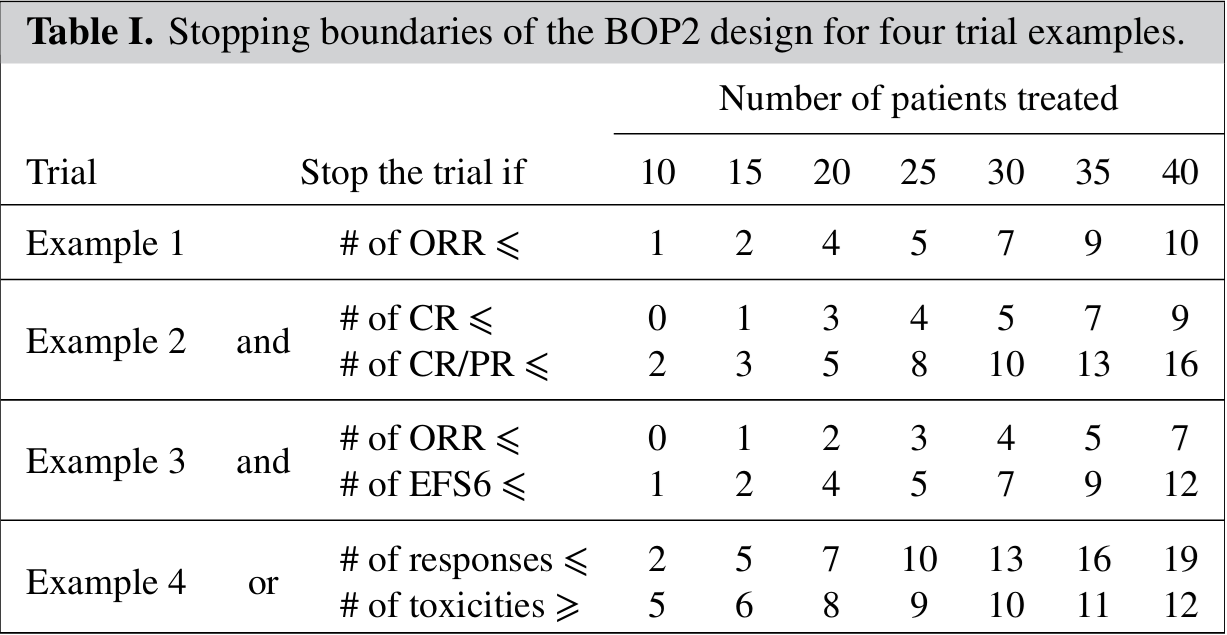
\includegraphics[scale=0.4]{table1.png}
    \caption{Stopping boundaries of the BOP2 design for four trial examples}
    \label{fig:data}    
\end{figure}

\textbf{註解:} 最大樣本量為40。I型誤差率為10\%。BOP2, Bayesian optimal phase II; ORR, 客觀緩解率; CR, 完全緩解; PR, 部分緩解; EFS6, 6個月無事件生存率。

與大多數現有的貝葉斯設計不同，這些設計假設一個恆定的臨界值，我們在此允許臨界值 \( C(n) \) 隨期中樣本量 \( n \) 變化。正如我們稍後所展示的，這種修改是重要的，並且顯著提高了設計的檢測能力。雖然這些停止規則有不同的臨床解釋，但「繼續/停止」決策都是基於模型參數 \( \theta = (\theta_1, \dots, \theta_K)^T \) 的線性組合的後驗機率進行評估，例如：

\[
\Pr(b\theta \leq \phi \mid D_n) > C(n),
\]

設計向量 \( b \) 的元素為 0 和 1，\( \phi \) 是一個預先設定的臨界值。例如，在試驗例2中，停止規則涉及評估兩個後驗機率，其中 \( b = (1, 0, 0, 0) \) 和 \( \phi = 0.15 \)，以及 \( b = (1, 1, 0, 0) \) 和 \( \phi = 0.3 \)；在試驗例3中，停止規則涉及評估兩個後驗機率，其中 \( b = (1, 1, 0, 0) \) 和 \( \phi = 0.1 \) 以及 \( b = (1, 0, 1, 0) \) 和 \( \phi = 0.2 \)。

評估公式(1)中的後驗機率可以通過利用狄利克雷分佈的以下性質來實現。

\textbf{性質 1}  
給定 \( \theta \sim \text{Dir}(a_1 + x_1, \dots, a_K + x_K) \) 和設計向量 \( b = (b_1, \dots, b_K) \)，其元素為 0 和 1，則 \( b\theta \) 服從參數為 

\[
\left( \sum_{k=1}^{K} b_k(a_k + x_k), \sum_{k=1}^{K} (1 - b_k)(a_k + x_k) \right)
\]

的貝塔分佈。

因此，可以方便地計算

\[
\Pr(b\theta \leq \phi \mid D_n) = B\left(\phi; \sum_{k=1}^{K} b_k(a_k + x_k), \sum_{k=1}^{K} (1 - b_k)(a_k + x_k)\right),
\]

其中 \( B(\phi; \zeta, \xi) \) 是參數為 \( \zeta \) 和 \( \xi \) 的貝塔分佈的累積分佈函數。這個 \( \Pr(b\theta \leq \phi \mid D_n) \) 的性質導致了以下結果。

***重點:

設計向量 b：設計向量 b 的每個元素可以是0或1，用來選擇模型參數 θ 的哪些部分將用於計算。在試驗過程中，不同的 b 向量可以用來對不同的組合結果進行檢驗。

臨界值 ϕ：這是一個預先設定的臨界值，用於決定在給定情況下是否應該停止試驗。

貝塔分佈：通過設計向量 b 的加權，所選擇的模型參數 θ 的組合 bθ 會服從貝塔分佈，這使得我們可以方便地計算出停止試驗的後驗機率。



\textbf{引理 1}
\[
\Pr(b\theta \leq \phi \mid D_n)
\]
是
\[
\sum_{k=1}^{K} b_k x_k
\]
的單調函數。

\( \Pr(b\theta \leq \phi \mid D_n) \) 的單調性在實踐中非常重要，因為它允許我們在試驗開始前列舉出停止邊界，類似於Simon的二階段設計，如表I所示。例如，‘例子2’中顯示了根據我們的試驗例子2中CR和CR/PR患者數量的期中停止邊界。在試驗進行過程中，我們不需要進行任何複雜的計算；我們只需要計算相關事件的數量，並根據該數量是否超過邊界來做出繼續/停止決策。例如，在治療了20名患者後，如果CR的反應數量 \(\leq 3\) 且CR/PR的反應數量 \(\leq 5\)，我們將提前終止試驗。這一特性使得BOP2設計在實踐中非常容易實施。


***重點:

引理1的意義：引理1表明，停止試驗的決策可以簡化為檢查某一特定加權和的單調函數是否超過了預設的臨界值，這使得停止邊界的設計和應用更加直接和方便。

實踐應用：在實際的臨床試驗中，研究者可以根據提前設定的停止邊界進行決策，而不需要進行複雜的計算。這使得BOP2設計不僅具有理論上的優勢，而且在實施上也更加容易和高效。

\subsection{Optimizing design parameters}

假設選擇了適當的虛無假設 \( H_0 \) 和備選假設 \( H_1 \) 來反映臨床研究的關注點，其中 \( H_0 \) 指定了治療被認為無效時參數 \( \theta \) 的取值，而 \( H_1 \) 則指定了治療被認為有效時 \( \theta \) 的取值。例如，在試驗例2中，\( H_0 \)：\( \theta_1 = 0.15 \) 且 \( \theta_1 + \theta_2 = 0.3 \)，合理的備選假設是 \( H_1 \)：\( \theta_1 = 0.25 \) 且 \( \theta_1 + \theta_2 = 0.5 \)。對於複雜的終點（例如，兩個共同主要終點），\( H_1 \) 的設定不太直觀，應通過與臨床醫生協商來確定，以反映實際可行且理想的結果。如果在整個試驗期間（包括試驗結束時）停止邊界從未被超過，我們拒絕 \( H_0 \) 並聲稱該治療具有前景。I型誤差率和統計檢測力分別定義為在 \( H_0 \) 和 \( H_1 \) 下拒絕 \( H_0 \) 的機率。

BOP2設計的運行特性依賴於機率臨界值 \( C(n) \) 的設定。雖然可以使用任何合理靈活的單調遞減函數 \( C(n) \)，但一個簡單且具有良好運行特性的二參數冪函數是：

\[
C(n) = 1 - \lambda \left(\frac{n}{N}\right)^\gamma,
\]

其中 \( \lambda \) 和 \( \gamma \) 是調整參數。我們要求 \( \gamma > 0 \)，使得 \( C(n) \) 隨 \( n/N \) 的增長單調遞減。其背後的理論是，在試驗初期，數據較少且不確定性較大，可能需要一個更為寬鬆的停止規則（即較大的 \( C(n) \)），以避免意外終止試驗。隨著試驗的進展和信息的積累，我們對於終點的不確定性減少，因此希望有一個更嚴格的停止規則（即較小的 \( C(n) \)），以終止對無效治療的試驗。剩下的問題是如何根據特定標準選擇調整參數 \( \lambda \) 和 \( \gamma \)，以及有時選擇 \( N \) 以優化設計的性能。

***重點:

虛無假設和備選假設：虛無假設H0通常代表治療無效，而備選假設 H1 則代表治療有效。在設計試驗時，需要明確這些假設的參數設定，以便於後續的統計檢驗。

I型誤差和檢測力：I型誤差率是指在 H0為真時錯誤拒絕 H0 的機率，而檢測力則是在 H1為真時正確拒絕H0的能力。

臨界值函數 C(n)：BOP2設計依賴於一個隨樣本量變化的臨界值函數 C(n)。文中推薦了一個簡單的二參數冪函數來表示該臨界值，這樣可以根據試驗進展動態調整停止規則。

調整參數的選擇：調整參數 λ 和 γ 的選擇是優化試驗設計的關鍵部分，需要根據具體的研究目標和試驗條件來確定。


我們首先考慮在樣本量 \( N \) 固定的情況下如何選擇調整參數 \( \lambda \) 和 \( \gamma \)，例如，由於預算有限或納入率受限。我們的策略是選擇 \( \lambda \) 和 \( \gamma \) 來最大化 BOP2 設計的檢測力，同時在某一預設水平上控制 I 型誤差率。具體步驟如下：

\textbf{步驟 1}：從臨床醫生處獲得 \( H_0 \) 和 \( H_1 \) 以及所需的 I 型誤差率。

\textbf{步驟 2}：找到產生所需 I 型誤差率的 \( (\lambda, \gamma) \) 值，這可以通過網格搜索來實現。

\textbf{步驟 3}：在步驟 2 中確定的 \( (\lambda, \gamma) \) 集合中，選擇一個使檢測力達到最大值的作為最優設計參數。

雖然 BOP2 設計是一種貝葉斯設計，但仍然需要確保該設計具有可接受的頻率學特性（例如，I 型誤差率和檢測力）。一般來說，一個好的貝葉斯設計應該展示出合理的頻率學運行特性\cite{source}. 明確控制 I 型誤差率是區分 BOP2 設計與大多數現有的貝葉斯第二期設計的一個重要特徵。這一特徵縮小了貝葉斯設計與頻率學設計之間的差距，使得 BOP2 設計對於廣泛的用戶和監管機構更易接受。


***重點:

調整參數 λ 和 γ：這些參數用來調整 BOP2 設計中的臨界值函數 C(n)，以實現對檢測力和 I 型誤差率的控制。

最大化檢測力：在選擇設計參數時，最優化的目標是提高檢測力，即在治療有效時能正確拒絕虛無假設 H0 的能力。

控制 I 型誤差率：在設計試驗時，控制 I 型誤差率至關重要，因為它涉及在治療無效時錯誤地接受治療效果的風險。

貝葉斯設計與頻率學設計的平衡：BOP2 設計的優勢在於它在保持貝葉斯設計靈活性的同時，也能夠展示出合理的頻率學特性，這使得該設計更容易被臨床和監管機構所接受。


一種替代優化策略是選擇 \( \lambda \) 和 \( \gamma \)，以及樣本量 \( N \)，以在給定的 I 型和 II 型誤差率下最小化虛無假設 \( H_0 \) 下的期望樣本量 \( E(N \mid H_0) \)。這種優化標準在 Simon 的最優設計中被使用。在這種方法中，\( N \) 不是固定的，而是要優化的設計參數。確定 \( (\lambda, \gamma, N) \) 值以最小化 \( E(N \mid H_0) \) 的過程可以描述如下：

\textbf{步驟 1}：從臨床醫生處獲得 \( H_0 \) 和 \( H_1 \) 以及所需的 I 型和 II 型誤差率。

\textbf{步驟 2}：找到 \( (N, \lambda, \gamma) \) 值以滿足所需的 I 型和 II 型誤差率，這可以通過網格搜索實現。

\textbf{步驟 3}：在步驟 2 中確定的 \( (N, \lambda, \gamma) \) 集合中，選擇一個使 \( E(N \mid H_0) \) 最小的作為最優設計參數。

在步驟 2 中，我們有兩個約束條件（即 I 型和 II 型誤差率），但需要確定三個未知參數 \( (N, \lambda, \gamma) \)。因此，理論上可能存在無限多的解決方案。我們通過將 \( N \) 的值限制在 \( (N_{\text{min}}, N_{\text{max}}) \) 範圍內來解決這個問題，其中 \( N_{\text{max}} \) 是實際上我們能夠承受的最大樣本量，通常由預算、納入率或其他實際因素決定。\( N_{\text{min}} \) 是試驗的最小樣本量，對於設計的運行特性影響不大，只要 \( N_{\text{min}} \) 合理地小，例如 \( N_{\text{min}} = 10 \)。給定一個具體的 \( N \) 值，我們可以通過網格搜索基於兩個約束條件唯一地確定 \( \lambda \) 和 \( \gamma \) 的值。這種優化策略的一個潛在限制是，我們無法直接控制樣本量 \( N \)，而且在某些情況下使 \( E(N \mid H_0) \) 最小的 \( N \) 值可能過大，實際使用中會存在困難。當這成為一個問題時，可以使用極大極小準則來優化設計。即，不是最小化 \( E(N \mid H_0) \)，而是選擇 \( (\lambda, \gamma, N) \) 以最小化最大樣本量。


***重點:

期望樣本量的最小化：這種策略旨在選擇合適的參數來最小化在虛無假設成立時的期望樣本量，這有助於提高試驗的效率，避免不必要的樣本浪費。

網格搜索：通過網格搜索來找到合適的 (λ,γ,N) 值，這是一種常見的優化方法，用於在給定條件下找到最佳參數組合。

極大極小準則：當最小化期望樣本量 E(N∣H 0) 導致的樣本量過大時，可以使用極大極小準則來優化設計，通過最小化最大樣本量來實現更加實用的設計。

\section{Webapplication}
\section{Simulation studies}

\end{document}

